
\documentclass[aps,prl,reprint]{revtex4-2}
\usepackage{gensymb}
\usepackage{graphicx}
\usepackage{amsmath}
\usepackage{hyperref}
\usepackage{dsfont}
\usepackage{relsize}
\usepackage{wrapfig}
\usepackage{graphicx}
\usepackage{hyperref}
\hypersetup{colorlinks=true, citecolor=blue, urlcolor=blue, linkcolor=blue}


\begin{document}

% Use the \preprint command to place your local institutional report
% number in the upper righthand corner of the title page in preprint mode.
% Multiple \preprint commands are allowed.
% Use the 'preprintnumbers' class option to override journal defaults
% to display numbers if necessary
%\preprint{}

%Title of paper
\title{Speed of Light Lab}

% repeat the \author .. \affiliation  etc. as needed
% \email, \thanks, \homepage, \altaffiliation all apply to the current
% author. Explanatory text should go in the []'s, actual e-mail
% address or url should go in the {}'s for \email and \homepage.
% Please use the appropriate macro foreach each type of information

% \affiliation command applies to all authors since the last
% \affiliation command. The \affiliation command should follow the
% other information
% \affiliation can be followed by \email, \homepage, \thanks as well.
\author{Trevor Smith, Alex Storrer}
\email[]{smith.tr@northeastern.edu}
\homepage[]{https://github.com/trevorm4x/}
%\thanks{}
%\altaffiliation{}
\affiliation{Northeastern University}


\date{\today}

\begin{abstract}
	Nothing is here
\end{abstract}


\maketitle

% body of paper here - Use proper section commands
% References should be done using the \cite, \ref, and \label commands
\section{Introduction}
% The Introduction should contain 1 or 2 paragraphs.
% Briefly state the physics underlying the experiment
% (what is being tested and why). 
The speed of light is foundational to our understanding of the universe, as it is in
fact not just the speed photons travel at, but rather a universal speed limit. 
However, even though photons do always travel at the speed of light, we can measure 
the net wavefront in a material at lower speeds, due to the absorption and re-emission
of new photons by atoms in a medium. This ``speed of light in a medium" is usually
thought of not as a speed, but as a ratio $v/c=n$, the refractive index. The 
refractive index is so called because light follows Snells law, where its direction
will be refracted proportional to this refractive index depending on the refractive
indeces of the two mediums.\\

It is, however, also useful to think of ``speed of light in a medium" as a speed, 
because the speed of communications in our incredibly connected world is crucial. 
Even electrical signals, governed by the electromagnetic force which is mediated by
photons, propogate through electrical circuits and cables not at the drift speed of
electrons but rather at the speed an electric field propogates through them. A major
advancement in communications, however, came from using photons themselves rather
than electrical signals to communicate over long distances, using Fiber-Optic (FO) 
cables. These cables take advantage of differences in the refractive index of glass
and another material to create total internal reflection of all photons input at the
end of a long and thin glass tube. These cables are capable of transmitting great 
amounts of information in a very thin tube, as, while conductors permit more 
information to flow through them limited by their circumference, FO cables use their
entire cross-sectional area to transmit information. \\

In this lab, we will measure the speed of light (and the effective speed of light) 
through different mediums, in order to calculate refractive index. The core technique
will involve using a laser and a beam splitter to pass two beams through paths of 
very different lengths, collecting the signals on two photodiodes (PD), and measuring
the relative delay of the longer path compared to the shorter one on an 0.5 GHz
oscilloscope. This laser will be triggered on and off with a nonosecond pulse 
generator. All factors: the pulse generator, the beam path lengths, the sample rate,
and the comparison between the two PD input signals for their time delay, will 
introduce sources of uncertainty that must be minimized by careful measurements and
signal processing. \\

The mediums considered will be air, glass (FO cable), and water. The effective 
index of the coax cables connecting the PD and oscilloscope will also be measured.


\section{Apparatus}
% List equipment components (manufacturer, model
% numbers and brief specifications). 

The apparatus consisted of the following.
\begin{itemize}
\item Oscilloscope, Tektronix TDS210
\item OpenChoice Desktop, Oscilloscope Software
\item Optical breadboard
\item Beam splitter, 2 mirrors, focusing lens
\item Focused laser diode
\item 2 Amplified high-speed silicon photodiodes
\item Water-Filled optical cell
\item Fast edge nanosecond pulse generator
\item Fiber Optic Cable with mount
\item BNC cables and male-male BNC connector
\item Spectrometer and Quantum software, Amadeus
\item Jupyter, Python compiler
\end{itemize}

\section{Procedures and Results}

\subsection{Test Pulse, Scope and Laser Diode}
% Briefly describe the experimental procedures (in your own words, but don’t overdo it)
% Discuss calibrations, etc., if required
% Include necessary equations and put them on their own line (number them, e.g. “Eq. (3)”)
% Include plots showing relevant results (label each figure, e.g. “Fig. 3”, with caption).
% Describe what you found (describe what the plot illustrates)
The  fast  edge  nanosecond  pulse  generator  uses  six74AC14 Schmitt Triggers as shown 
in fig. \ref{Schmitt}, hand mounted to a copper circuit board.\\

\begin{figure}[h]
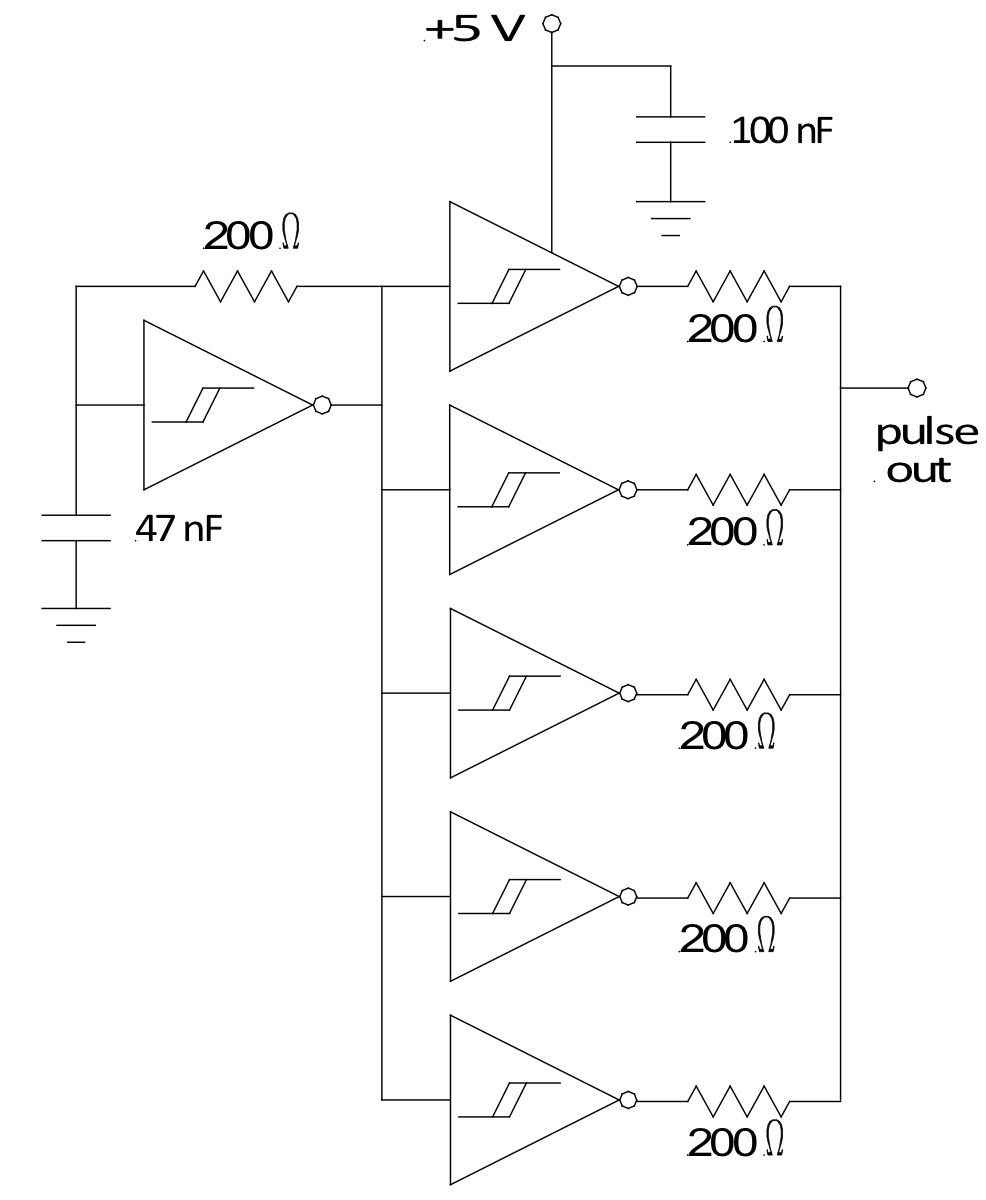
\includegraphics[width=0.4\textwidth]{./BMPs/Schmitt.jpg}
\caption{\label{Schmitt} Circuit diagram of the nanosecond pulse generator}
\end{figure}

The pulse generator was connected directly to the oscilloscope, and adjusted until
several cycles were visible on the display. This output was analyzed to verify the setup.
These square pulses are shown in fig. \ref{squares}. We can observe an approximate 
amplitude of 5.60 mV, and using fourier analysis we can verify that the fundamental 
frequency is 90 kHz. \\

\begin{figure}[h]
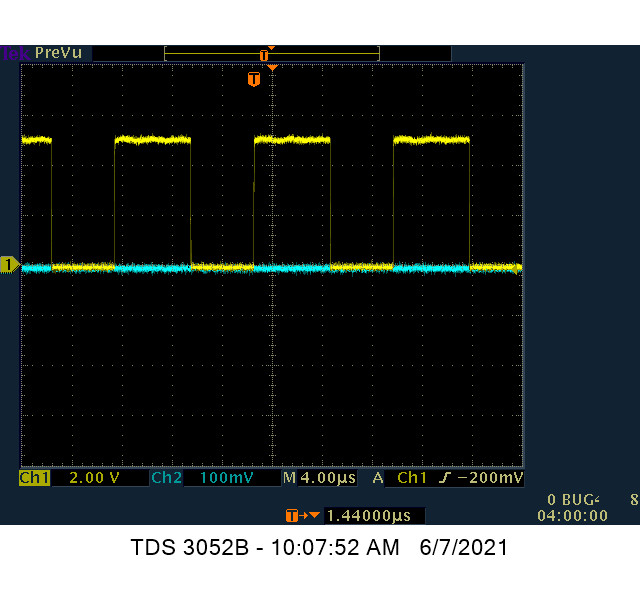
\includegraphics[width=0.4\textwidth]{./BMPs/l4_A_1.jpg}
\caption{\label{squares} Measured square waves on the oscilloscope.}
\end{figure}

The pulse generator will be used to power the laser, creating a wave
front that propogates simultaneously through two paths of different lenghts. \\


\subsection{Optical Setup}

Next, the two paths were configured, based on \ref{setup}. We will consider only the
distances of the paths after the beam splitter, as the paths up until that point are
equivalent. The path measured by PD1 is given by length 1 alone, and the path measured
by PD2 is given by lengths 2-5. These lengths are given in \ref{SetupLengths}, with
all measurements performed with a tape measure.
After completing all measurements in the span of two days,
a final re-demonstration of the lab was performed in a single day, and it is these results
that are shown below, with the geometry of the setup unchanged for the entirety of the 
lab. \\

\begin{figure}[h]
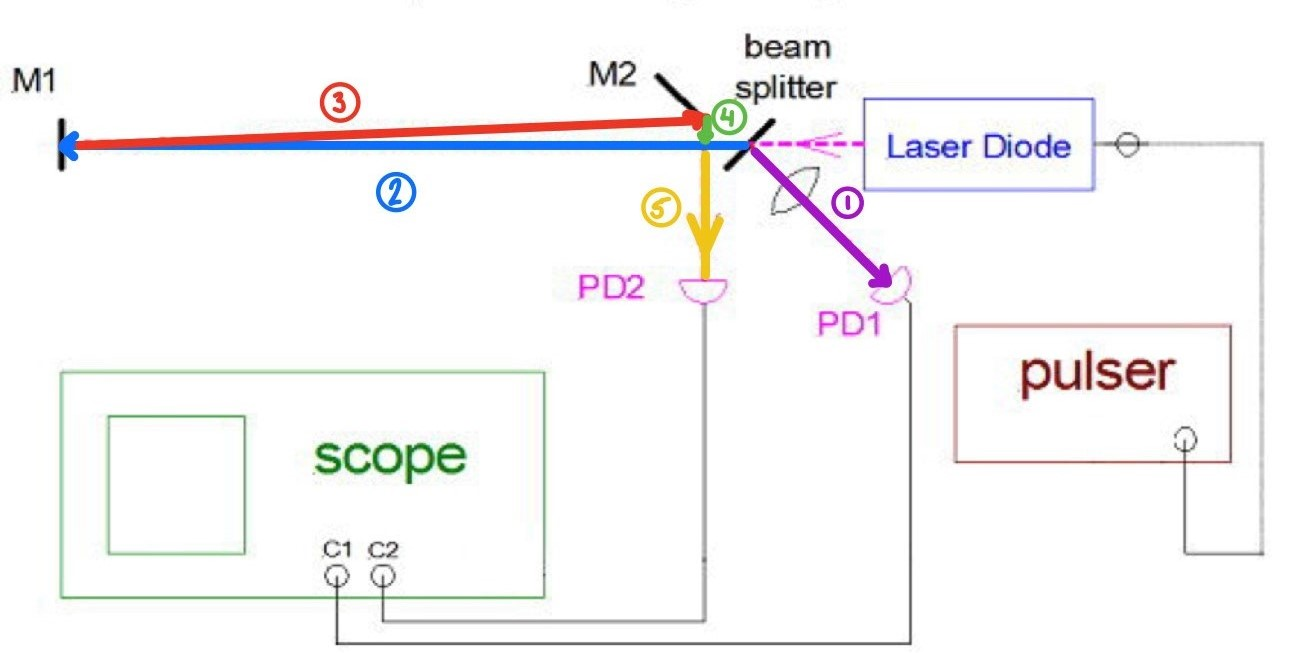
\includegraphics[width=0.4\textwidth]{./BMPs/Optical Setup.jpg}
\caption{\label{setup} Annotated test setup.}
\end{figure}

\begin{table}[h]
\renewcommand{\arraystretch}{1.35}
\setlength{\tabcolsep}{10pt}
\caption{\label{SetupLengths}Lengths of various paths shown the optical setup}
\begin{tabular}{|c|c|c|}
	%\hline
	\toprule
	length \# & Color & Length (mm)\\
	\colrule
	1 & Purple & 168.5\\
	\colrule
	2 & Blue & 917.5\\
	\colrule
	3 & Red & 730.0\\
	\colrule
	4 & Green & 5.0\\
	\colrule
	5 & Mustard & 124.5\\
	\hline
	\botrule
\end{tabular}
\end{table}

Before measuring distances PD1 and PD2 were connected to the oscilloscope, and the signal
was isolated on the oscilloscope, triggered by PD1, as shown in 
\ref{setup}, where a visible time shift can be observed.
By referencing the oscilloscope output, the setup was optimized for the
strongest signal by adjusting the beam splitter and M2. \\

\begin{figure}[h]
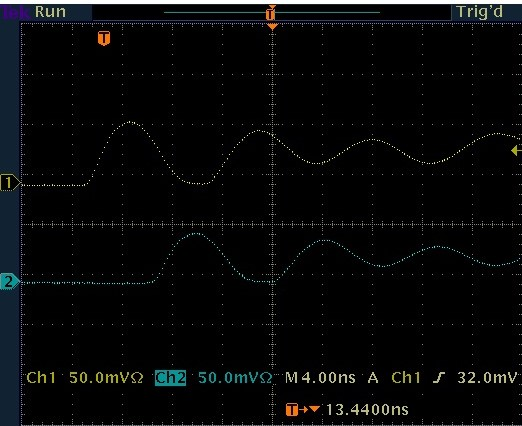
\includegraphics[width=0.45\textwidth]{./BMPs/l4_C_b.jpg}
\caption{\label{setup} Oscilloscope output for test setup with equal length BNC cables.
Signals PD1 and PD2 are labeled on the left 1 and 2 respectively.}
\end{figure}

Measurements were then recorded for analysis, as shown in fig. \ref{same}. It should be
noted that for a perfect experimental setup, these signals would appear as simple step
functions or square waves. However, producing such a sharp signal is very difficult,
and as such more detailed analyis must be done to compare the two signals than simply 
looking at the step time. The ``10-90" rise times were used to compare flight times of 
the two signals, in addition to the min and max of the signals. These values are shown
in table \ref{TD_Ca}. \\

\begin{figure}[h]
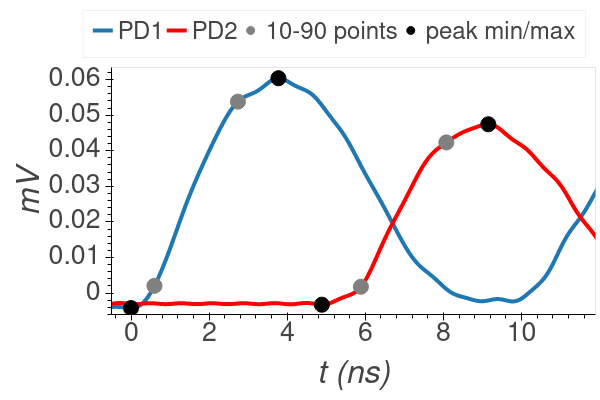
\includegraphics[width=0.45\textwidth]{../Images/l4_C_b.png}
\caption{\label{same} Oscilloscope data comparing reference points for PD1 and PD2.}
\end{figure}

From table \ref{TD_Ca}, the time delay between PD1 and PD2 was calculated, with the
mean and the standard deviation being taken as the recorded measurement and 
uncertainty, at 5.2 $\pm$ 0.2 ns. The high uncertainty in this measurement can
be attributed to the difference in the peak shapes, where the full-width half-max (FWHM)
for PD1 was calculated to be 4.657 ns, and the FWHM for PD2 was calculated to be 4.534 ns.
This error is compensated for in future measurements, but in this case is less relevant. \\

\begin{table}[h]
\renewcommand{\arraystretch}{1.35}
\setlength{\tabcolsep}{10pt}
\caption{\label{TD_Ca}Time values of the first nanosecond peaks for equal length BNC cables}
\begin{tabular}{|c|c|c|c|c|}
%\hline
\toprule
PD & Start & End & 10\% & 90\% \\
\# & (ns)& (ns)& (ns)& (ns)\\
\colrule
1 &    0.0 &  2.47 &  0.67 &  2.02 \\
\colrule
2 &    5.4 &  7.79 &  5.97 &  7.27 \\
\hline
\botrule
\end{tabular}
\end{table}

Next, the BNC cable connecting PD2 to the oscilloscope, which originally was of equal 
length to the cable connecting PD1, was replaced with a significantly longer cable in order
to explore such a scenario, and calculate the effective refractive index of the BNC
cables. The scope output is shown in \fig. \ref{diff}, and the graph with reference points 
included is shown in fig. \ref{setup2}. The values for the 10-90 rise time, min, and max are
shown in table \ref{TD_Cb}. \\


\begin{figure}[h]
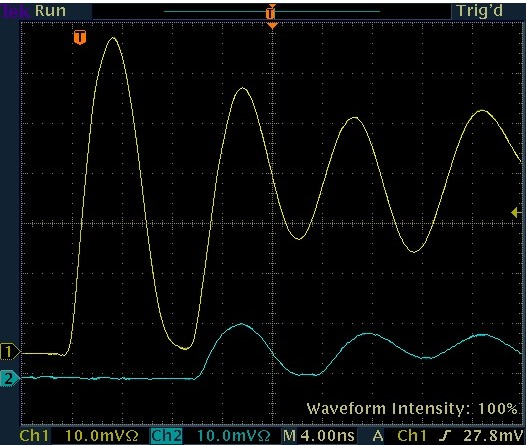
\includegraphics[width=0.45\textwidth]{./BMPs/l4_C_c.jpg}
\caption{\label{setup2} Oscilloscope output for test setup with different length BNC cables.
Signals PD1 and PD2 are labeled on the left 1 and 2 respectively.}
\end{figure}

\begin{figure}[h]
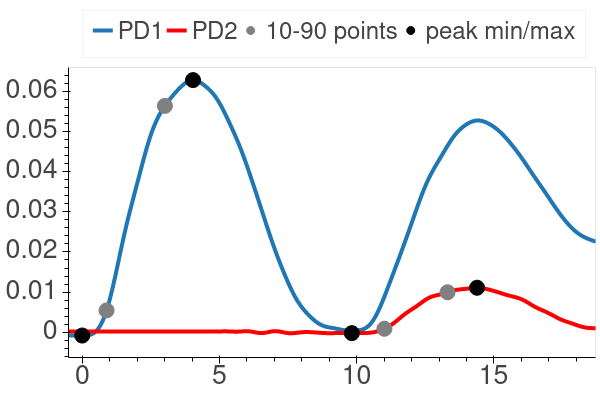
\includegraphics[width=0.45\textwidth]{../Images/l4_C_a.png}
\caption{\label{diff} Oscilloscope data comparing reference points for PD1 and PD2, where PD2 
has been delayed using a longer BNC cable.}
\end{figure}

\begin{table}[h]
\renewcommand{\arraystretch}{1.35}
\setlength{\tabcolsep}{10pt}
\caption{\label{TD_Cb} Time values of the first nanosecond peaks for different length 
	BNC cables}
\begin{tabular}{|c|c|c|c|c|}
%\hline
\toprule
PD & Start & End & 10\% & 90\% \\
\# & (ns)& (ns)& (ns)& (ns)\\
\colrule
1 &   0.00 &   4.04 &   0.89 &   3.01 \\
\colrule
2 &   9.82 &  14.39 &  11.01 &  13.31 \\
\hline
\botrule
\end{tabular}
\end{table}







A plot showing both sets of captures, with extra
cable and without extra cable, is sown in fig. \ref{comparison}. The extra delay due to
the extra cable length can be seen clearly.

\begin{figure}[h]
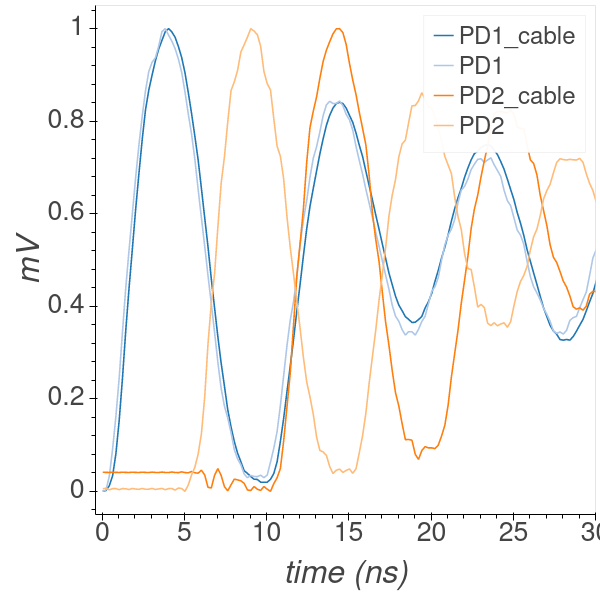
\includegraphics[width=0.45\textwidth]{./l4_A.png}
\caption{\label{comparison} Normalized comparison of the signals from PD1 and PD2 for equal
length cables as well as the inequal length cables, denoted by the suffix ``\_cable".}
\end{figure}






\newpage

\begin{equation}
    \mathlarger{\eta_{PV}}=P_E/P_L
    \label{eta_PV}
\end{equation}

\subsection{Conclusions}

\section{Summary}

\begin{widetext}
\begin{center}
\begin{table}[h]
\renewcommand{\arraystretch}{1.35}
\setlength{\tabcolsep}{10pt}
\caption{\label{}Measured and accepted values of the speed of light and refractive index of various materials.}
\begin{tabular}{|c|c|c|c|c|}
%\hline
\toprule
Apparatus &  $\eta$ (\%) & Accepted $\eta$ value & Refs. & Deviation \\
\colrule
Photovoltaic Cell &  $15 \pm 2$ & $17 \pm 2.5$ & \cite{Solar Cell} & $0\sigma$  \\
\colrule
Elecrolyzer &  $87 \pm 6$ & 80 & \cite{Electrolyzer} & $2\sigma$  \\
\colrule
Hydrogen Fuel Cell &  $49 \pm 5$ & 60 & \cite{Fuel Cell} & $-3\sigma$  \\
%\hline
\botrule
\end{tabular}
\end{table}
\end{center}
\end{widetext}





\begin{thebibliography}{9}
%
\bibitem{HHV} 
Wikipedia, Heat of Combustion: \\
\href{https://en.wikipedia.org/wiki/Heat_of_combustion}{https://www.wikepedia.com}
%
\bibitem{Solar Cell} 
Energysage, Most Efficient Solar Panels\\
\href{https://news.energysage.com/what-are-the-most-efficient-solar-panels-on-the-market/#:~:text=How%20efficient%20are%20solar%20panels,are%20not%20above%2020%25%20efficiency.}{https://www.energysage.com/}
%
\bibitem{Electrolyzer} 
Carbon Commentary, Hydrogen made by Electolysis\\
\href{https://www.carboncommentary.com/blog/2017/7/5/hydrogen-made-by-the-electrolysis-of-water-is-now-cost-competitive-and-gives-us-another-building-block-for-the-low-carbon-economy}{https://www.carboncommentary.com}
%

%
\bibitem{Fuel Cell} 
Energy.gov, Fuel Cell Fact Sheet\\
\href{https://www.energy.gov/sites/prod/files/2015/11/f27/fcto_fuel_cells_fact_sheet.pdf}{https://www.energy.gov}

\end{thebibliography}


\end{document}
%
% ****** End of file apstemplate.tex ******

